% MplTplt - Yet another LaTeX template for Modern Physics Lab, PKU.
% Copyright (C) 2014 Huang Kangjing and contributors

% This work is completely rewritten basing on the work of Cao Chuanwu
% and Sun Sibai, with texts in the template originally coming from the
% Modren Phys. Lab.

% This file is released under the MIT license.
%
% Permission is hereby granted, free of charge, to any person obtaining a copy
% of this software and associated documentation files (the "Software"), to deal
% in the Software without restriction, including without limitation the rights
% to use, copy, modify, merge, publish, distribute, sublicense, and/or sell
% copies of the Software, and to permit persons to whom the Software is
% furnished to do so, subject to the following conditions:
% 
% The above copyright notice and this permission notice shall be included in
% all copies or substantial portions of the Software.
% 
% THE SOFTWARE IS PROVIDED "AS IS", WITHOUT WARRANTY OF ANY KIND, EXPRESS OR
% IMPLIED, INCLUDING BUT NOT LIMITED TO THE WARRANTIES OF MERCHANTABILITY,
% FITNESS FOR A PARTICULAR PURPOSE AND NONINFRINGEMENT. IN NO EVENT SHALL THE
% AUTHORS OR COPYRIGHT HOLDERS BE LIABLE FOR ANY CLAIM, DAMAGES OR OTHER
% LIABILITY, WHETHER IN AN ACTION OF CONTRACT, TORT OR OTHERWISE, ARISING FROM,
% OUT OF OR IN CONNECTION WITH THE SOFTWARE OR THE USE OR OTHER DEALINGS IN
% THE SOFTWARE.
%

% This template depends on the "revtex4.1" package from APS Journals
% <http://publish.aps.org/revtex/revtex-faq>, and the Chinese handling
% is done with XeLaTeX engine and package "xeCJK". Please ensure these
% packages are available in your chosen Tex software distribution.

% Document created using this template should be compiled with XeLaTeX
% engines rather than plain LaTeX or plain TeX engines.

% The non-ASCII texts of this template is encoded in UTF-8 encoding.
% Please note that XeLaTeX only accepts UTF-8 encoded documents, so
% set your editor to use UTF-8 while creating documents with this template.

% Recommended TeX software distribution to use with this template is
% Tex Live developed by the TeX User Group (TUG), please visit the home
% page of the distribution <https://www.tug.org/texlive/> for further details.

% NOTE THAT IMPORTANT INSTRUCTIONS HAS BEEN WRITTEN AS UPPERCASE COMMENTS
% IN THE TEXT, PLEASE READ THEM CAREFULLY AND FOLLOW THEM TO MAKE THE
% TEMPLATE WORK!

% Any further contributions to the template is welcome, please send
% pull requests through github or send mail to maintainer.

% For any other questions, please do not hesitate to contact maintainer.

% Current maintainer:
% Huang Kangjing <huangkangjing@gmail.com>

% Contributors:
% Sun Sibai <niasw@pku.edu.cn>
% Cao Chuanwu <>
% Huang Kangjing <huangkangjing@gmail.com>


\documentclass[aps,pre,12pt,preprint,onecolumn,showpacs,showkeys,floatfix]{revtex4-1}

% Setting up Chinese handling.
\usepackage{fontspec,xeCJK}

% Setting up fonts.
% PLEASE MODIFY ALL THESE FONT NAMES ACCORDING TO YOUR FONT
% INSTALLATION AND PERFERENCE.

% Setting up main fonts and mono fonts.
\setmainfont{Liberation Serif}
\setmonofont{Liberation Mono}
% SimSun is required font for the main body of the text.
\setCJKmainfont[AutoFakeBold=5,AutoFakeSlant]{SimSun}
\setCJKmonofont[AutoFakeBold=2,AutoFakeSlant]{SimHei}

% Setting up alternative font families.
% Note that these three fonts below are required fonts in document
% title, section headings and figure captions.
\newCJKfontfamily\heiti[AutoFakeBold=2,AutoFakeSlant]{SimHei}
\newCJKfontfamily\fangsong[AutoFakeBold=5,AutoFakeSlant]{FangSong}
\newCJKfontfamily\kaiti[AutoFakeBold=5,AutoFakeSlant]{KaiTi}

% Setting up paragraph indent.
\parindent 2em

% Setting up macros for Chinese-style font size setting.
\newcommand{\fseight}{\fontsize{5.02}{6.02}\selectfont}
\newcommand{\fsseven}{\fontsize{5.52}{6.62}\selectfont}
\newcommand{\fsssix}{\fontsize{6.52}{7.83}\selectfont}
\newcommand{\fssix}{\fontsize{7.53}{9.03}\selectfont}
\newcommand{\fssfive}{\fontsize{9.03}{10.84}\selectfont}
\newcommand{\fsfive}{\fontsize{10.54}{12.65}\selectfont}
\newcommand{\fssfour}{\fontsize{12.05}{14.45}\selectfont}
\newcommand{\fsfour}{\fontsize{14.05}{16.86}\selectfont}
\newcommand{\fssthree}{\fontsize{15.06}{18.07}\selectfont}
\newcommand{\fsthree}{\fontsize{16.06}{19.27}\selectfont}
\newcommand{\fsstwo}{\fontsize{18.07}{21.68}\selectfont}
\newcommand{\fstwo}{\fontsize{22.08}{26.50}\selectfont}
\newcommand{\fssone}{\fontsize{24.09}{28.91}\selectfont}
\newcommand{\fsone}{\fontsize{26.10}{31.32}\selectfont}
\newcommand{\fsszero}{\fontsize{36.14}{43.36}\selectfont}
\newcommand{\fszero}{\fontsize{42.16}{50.59}\selectfont}

% Replace words to Chinese corespondence.
\renewcommand\appendixname{附录}
\renewcommand\abstractname{}
\renewcommand\tablename{表}
\renewcommand\figurename{图}

% Replace words in revtex4-1 to Chinese corespondence.
\makeatletter
\def\@pacs@name{\heiti\fssfour \textbf{PACS码:}\normalfont}
\def\@keys@name{\heiti\fssfour \textbf{关键词:}\normalfont}
\def\Dated@name{日期:}
\def\Received@name{\fssfive 接收 }
\def\Revised@name{\fssfive 修订 }
\def\Accepted@name{\fssfive 采纳 }
\def\Published@name{\fssfive 发表 }
\makeatother

% Change label style of enumerate.
\renewcommand{\labelenumi}{\alph{enumi}.}

% Setting up geometry.
\usepackage{geometry}
\geometry{top=2.54cm,bottom=2.54cm,left=3cm,right=3cm}

% Setting up line space.
\usepackage{setspace}
\linespread{1.6}

% Setting up hyperreferences.
\usepackage{hyperref}
\hypersetup{colorlinks=true}

% Setting up styles for section headings.
\usepackage{titlesec}
\titleformat*{\section}{\bf\fangsong\fsfour}
\titleformat*{\subsection}{\bf\fangsong}

% Loading packages for image handling.
\usepackage{subfig}
\usepackage{graphicx,psfrag,epsfig}

% Setting up caption styles.
\usepackage{caption}
\DeclareCaptionFont{kaiti}{\kaiti}
\DeclareCaptionFont{bfheiti}{\bf\heiti}
\captionsetup{font=small,format=plain,labelfont=bfheiti,%
  textfont=kaiti,justification=raggedright,%
  singlelinecheck=false}

% Loading packages for math typings.
\usepackage{amsmath,amsfonts,amssymb,amsthm,bm,upgreek}
\usepackage[mathscr]{eucal}
\usepackage{siunitx}


\begin{document}

% Title and author info.
\title{\bf\heiti\fsthree 非线性对流斑图\vspace{15mm}}
\author{\fangsong\fsfour 黄康靖\vspace{2mm}}
\affiliation{\normalfont\fssfour 2012级~~~~学号:{masked student id}\vspace{2mm}}
\date{May 20th, 2015}
\keywords{非线性对流,耗散结构,非平衡态,贝纳问题}
\email{huangkangjing@gmail.com}

% Abstract.
\begin{abstract}
  \vspace{10mm}
  \begin{spacing}{1.5}
    \fssfour
    自然界中和人们的生活中充斥着不平衡过程,科学研究不平衡过程的理论是耗散结构理
    论.耗散结构理论是在20世纪60年代末由普利高津等人发展起来的科学理论,在自然和人
    文科学的各个领域都有着重要的应用.耗散结构理论的典型应用体系是贝纳问题的物理
    体系,即夹在两个温度不同的水平平面间的液体的热对流问题.本实验通过对于这一问题
    产生的非线性对流图样,即非线性对流斑图的观测,探索了相关的物理机制.
  \end{spacing}
\end{abstract}

% The main body of the document goes from here.
\maketitle
\fssfour

\section{引言}

当流体的内部密度压力分布不均匀产生梯度力时,流体便会发生流动.而当热力作用使得流体
状态(比如密度、压力等)发生的差异,也可以导致流体运动.这种由热力作用驱动的流体运动
称为热对流.它是自然界中常见的现象.热对流现象是由于热力分布的不均匀,造成了流体中
的温差,从而引起了流体的密度差,进而在重力场中相应地出现了阿基米德浮力驱动的.

1900年,贝纳对具有自由面-固壁底层的液体薄层进行了热对流实验,观测到了各种对流图形.
现在把底层加热的液体薄层的对流奋蹄称为贝纳问题,耗散结构理论的提出使得人们对于此
类问题有了更系统而深入的认识.

耗散结构理论是在20世纪60年代末由以普利高津为首的比利时布鲁塞尔学派提出的科学理论
,它给出了对于不可逆过程的科学研究方法.耗散结构理论指出,系统从无序状态过渡到耗散
结构有两个必要条件,一是系统必须开放,即系统必须与外界进行物质或能量的交换;二是系
统必须远离平衡态,即系统中流与力的关系是非线性的.

贝纳问题中的非线性对流结构是典型的耗散结构,对于其的研究有助于对于耗散结构理论的
进一步理解.本实验通过对于贝纳问题中过的非线性对流结构的表征形态非线性对流斑图的
形成过程的研究,对于耗散结构理论进行了探索.

\section{原理}

研究在上下相隔$d$的两个平面之间所夹住的一薄层液体中的热对流现象.上下两边界为水平,温度分别维持
为$T$和$T+\Delta T$($\Delta T > 0$).这一热对流系统满足Boussinesq条件,相应的热对
流基本方程组和边界条件如下

\begin{equation}
    \begin{cases}
        \frac{\partial \vec{V}}{\partial t} + \vec{V} \cdot \nabla\vec{V} =
        g\alpha T\hat{z} - \frac{1}{\rho}\nabla p + \gamma\nabla^2\vec{V} \\
        \nabla\cdot\vec{V} = 0 \\
        \frac{\partial \theta}{\partial t} + \vec{u}\cdot\nabla\theta =
        \kappa\nabla^2 T
    \end{cases}
\end{equation}

\begin{equation}
    \begin{cases}
        T(z = -d/2) = T + \Delta T \\
        T(z = d/2) = T \\
        \vec{V} = 0, z = \pm d/2
    \end{cases}
\end{equation}

对于这一定解问题可以做线性稳定性分析,通过对定态解施加围绕,讨论微扰的线性发展.

理论推导给出的结果指出,参数$R$瑞利系数
\begin{equation}
    R = \frac{g\alpha d^3\Delta T}{\kappa\gamma}
\end{equation}
是决定系统非线性特性的重要参量.数值计算结果则给出,$R$存在临界值
\begin{equation}
    R_c = 1707.76, \alpha_c = 3.117
\end{equation}
即是说,当系统的条件可以满足$R<R_c$时, 系统出现的随机扰动噪声会随时间演化消失,从
而不会出现非线性对流现象;而系统的条件满足$R>R_c$时,系统出现的随机扰动的非线性效
应将不会能够忽略,从而将会出现非线性对流现象与非线性斑图.

\section{实验}

在实验中,待测的液体水被夹在降温水层和纯紫铜盘的镀金表面之间.使用不同厚度的垫圈
垫在两个表面之间,来实现调整研究的液体水层的厚度.

降温水层与研究的液体水层的接触面
是蓝宝石片,其他部分是有机玻璃,降温水层内的水由水泵驱动,由制冷机保证其温度一直处
于某个较低的值.

下表面的纯紫铜盘上镀了一层金,用于反射光线,方便阴影法观测.紫铜盘内有电热丝和控温
器,用于保证其温度一直处于某个较高的值.

纯紫铜盘和降温水层中都有Pt100温度探测头,用于测量两侧的平面的温度.

实验采用阴影法来观测对流水层内的流动结构,即斑图.使用激光器作光源,经扩束镜扩束后,
再经凸透镜形成准平行光束,照射到水层上,收集反射的光线,使用CCD成像,用计算机拍照,即
可观测到斑图.

实验先后测量了$d = \SI{2}{mm}$,$d = \SI{4}{mm}$下,增加上下表面的温度差时,稳定斑
图的演化过程.

\section{实验结果及分析讨论}

斑图在两个不同的水层厚度下,演化的过程如以下诸图所示.

\begin{center}
    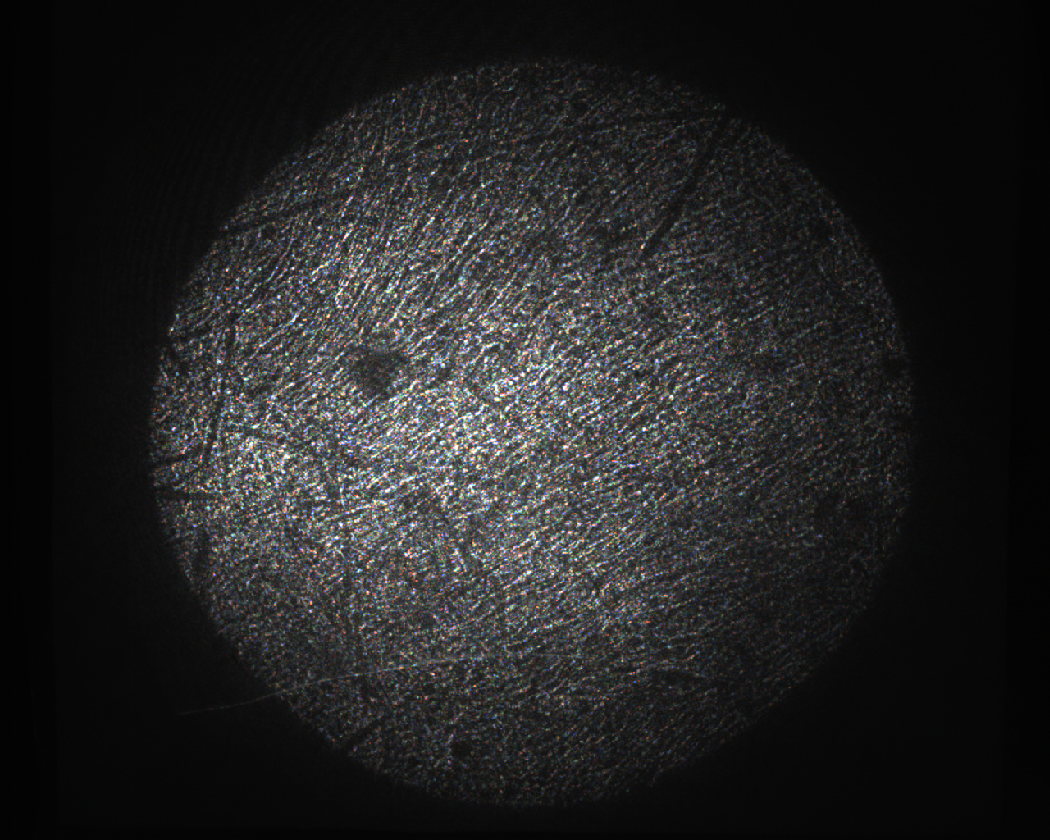
\includegraphics[width=.5\textwidth]{5.20/1.pdf}
\end{center}
    此图为厚度$d=\SI{2}{mm}$,加热电流$I=\SI{0.5}{A}$, 下界面温度为27.7摄氏度, 上界面温度为22.4摄氏
    度时的斑图图样,可以看到,此时非线性对流尚未形成.


\begin{center}
    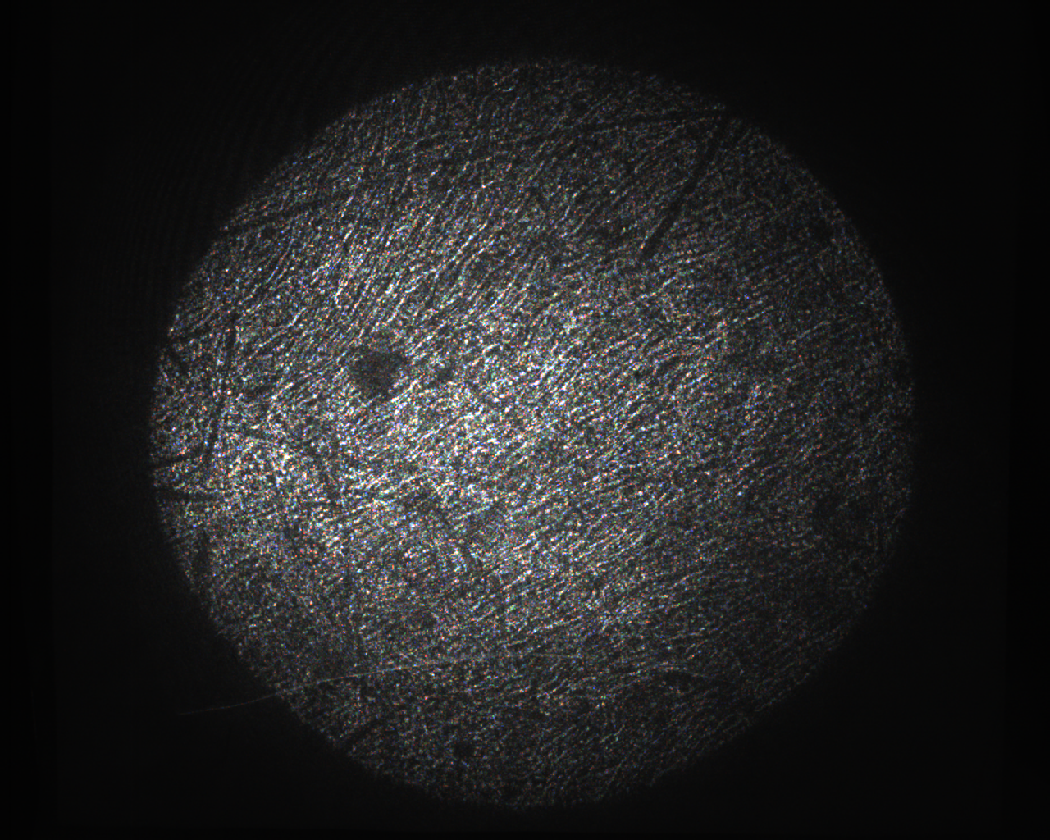
\includegraphics[width=.5\textwidth]{5.20/2.pdf}
\end{center}
    此图为厚度$d=\SI{2}{mm}$,加热电流$I=\SI{0.55}{A}$, 下界面温度为28.5摄氏度, 上界面温度为22.9摄氏
    度时的斑图图样,可以看到,此时非线性对流已开始形成,可以看到隐约的黑白相间条纹.

\begin{center}
    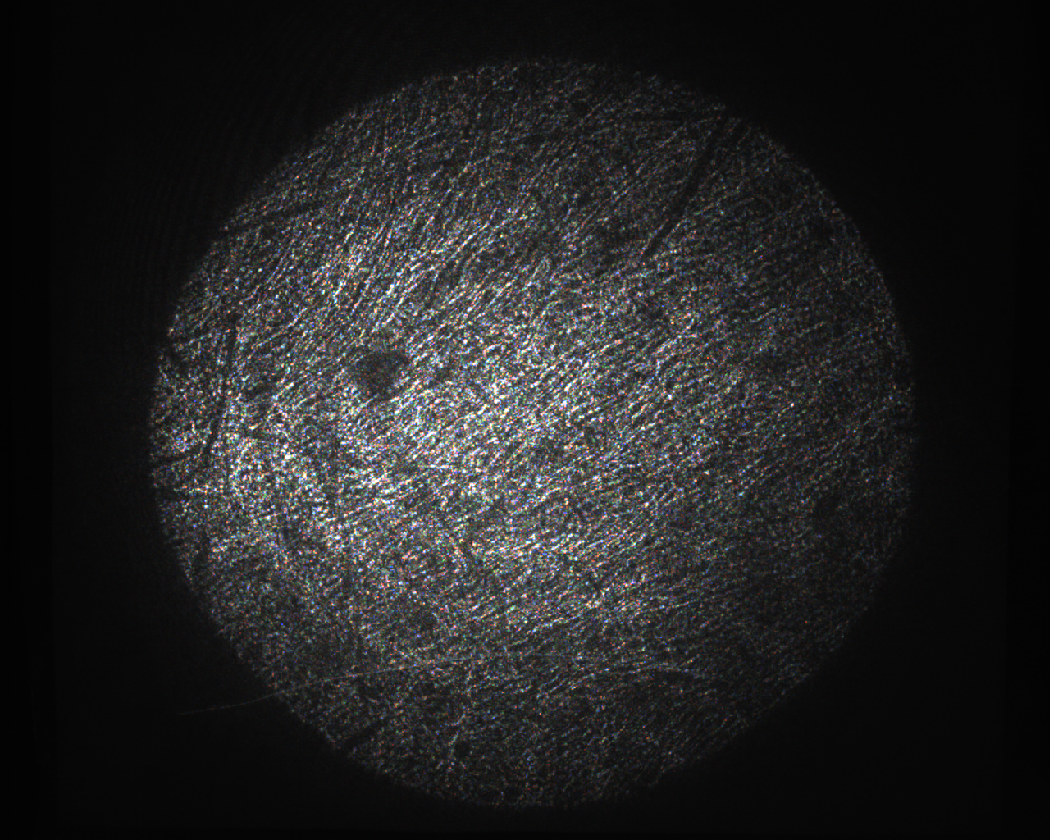
\includegraphics[width=.5\textwidth]{5.20/3.pdf}
\end{center}
    此图为厚度$d=\SI{2}{mm}$,加热电流$I=\SI{0.6}{A}$, 下界面温度为29.8摄氏度, 上界面温度为24.0摄氏
    度时的斑图图样,可以看到,此时斑图变得更加明显.

\begin{center}
    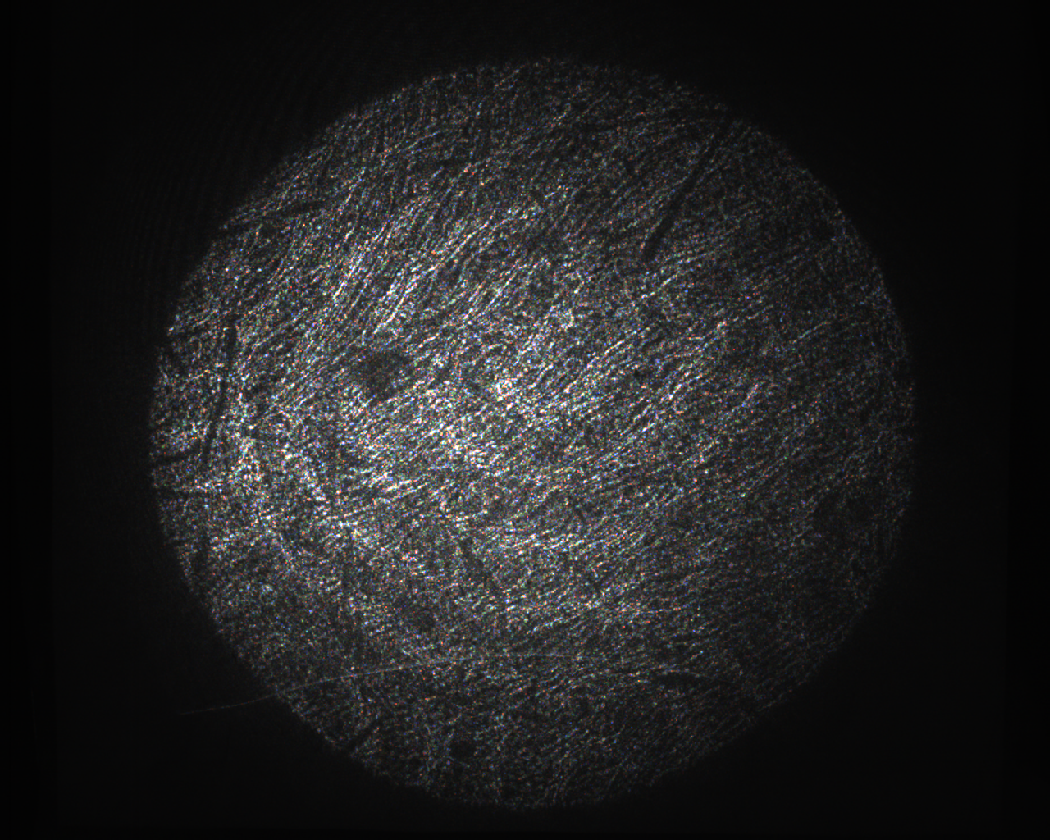
\includegraphics[width=.5\textwidth]{5.20/4.pdf}
\end{center}
    此图为厚度$d=\SI{2}{mm}$,加热电流$I=\SI{0.65}{A}$, 下界面温度为30.7摄氏度, 上界面温度为24.3摄氏
    度时的斑图图样,可以看到,此时斑图变得更加明显.

\begin{center}
    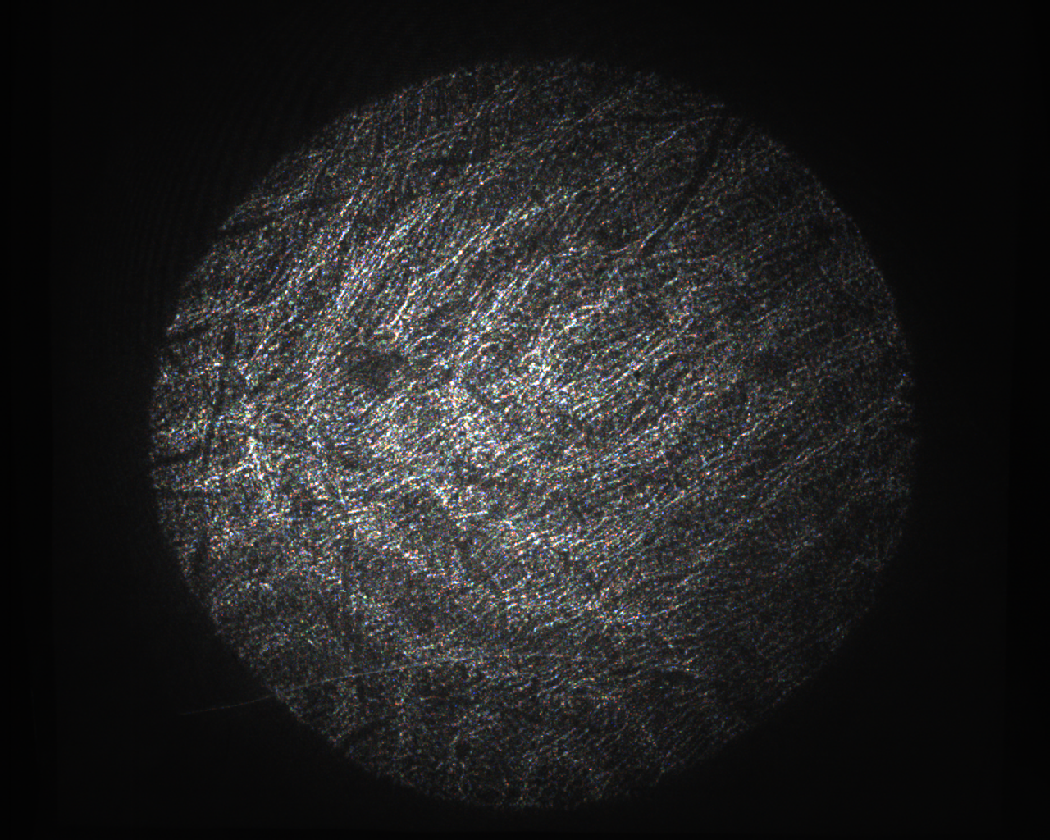
\includegraphics[width=.5\textwidth]{5.20/5.pdf}
\end{center}
    此图为厚度$d=\SI{2}{mm}$,加热电流$I=\SI{0.7}{A}$, 下界面温度为31.8摄氏度, 上界面温度为24.8摄氏
    度时的斑图图样,可以看到,此时斑图变得更加明显.

\begin{center}
    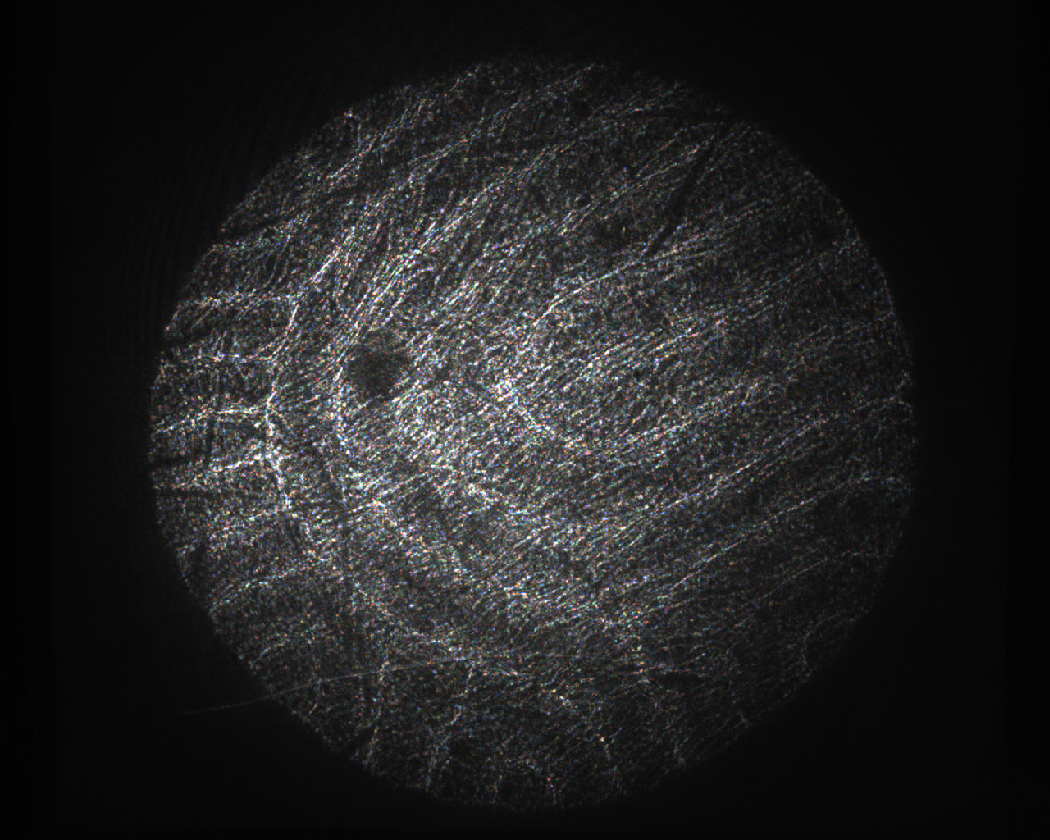
\includegraphics[width=.5\textwidth]{5.20/6.pdf}
\end{center}
    此图为厚度$d=\SI{2}{mm}$,加热电流$I=\SI{0.8}{A}$, 下界面温度为34.0摄氏度, 上界面温度为25.7摄氏
    度时的斑图图样,可以看到,此时斑图变得更加明显,并且出现了明确的白线边界.

\begin{center}
    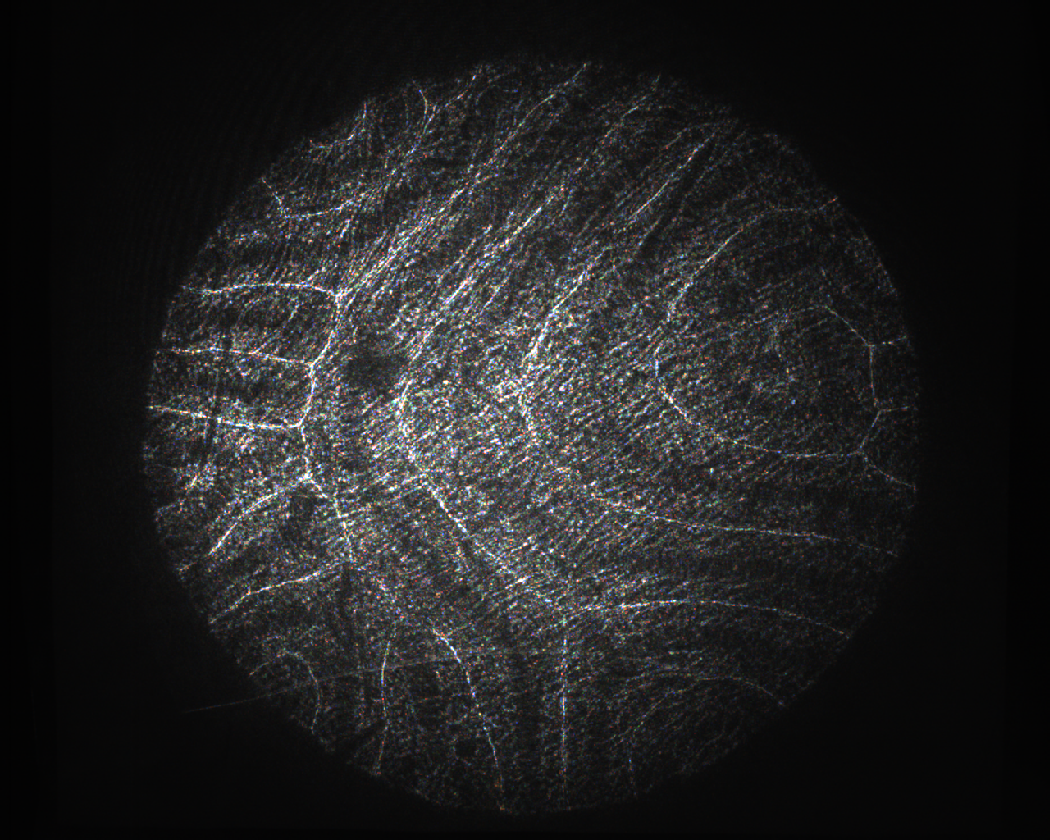
\includegraphics[width=.5\textwidth]{5.20/7.pdf}
\end{center}
    此图为厚度$d=\SI{2}{mm}$,加热电流$I=\SI{1.0}{A}$, 下界面温度为40.8摄氏度, 上界面温度为29.2摄氏
    度时的斑图图样,可以看到,此时斑图变得更加明显,并且出现了明确的黑线边界,图样有
    所变形.

\begin{center}
    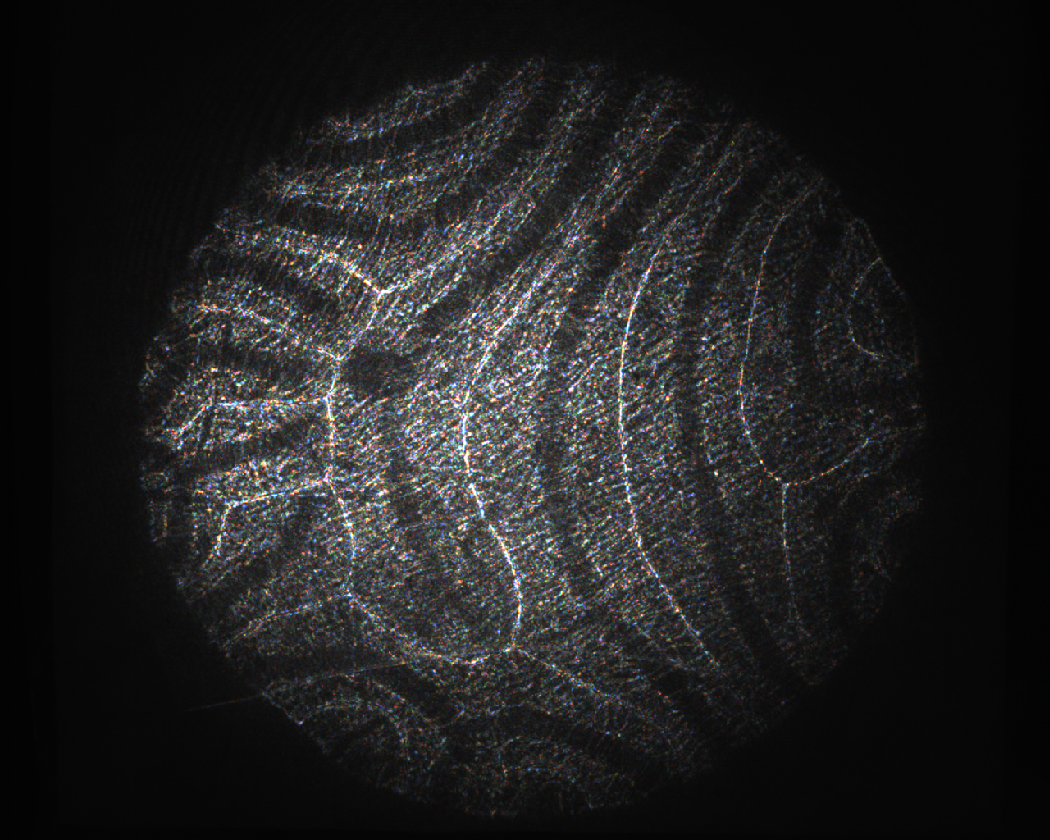
\includegraphics[width=.5\textwidth]{5.20/8.pdf}
\end{center}
    此图为厚度$d=\SI{2}{mm}$,加热电流$I=\SI{1.2}{A}$, 下界面温度为47.4摄氏度, 上界面温度为32.8摄氏
    度时的斑图图样,可以看到,此时斑图变得更加明显,斑图的变形也进一步增强了.

\begin{center}
    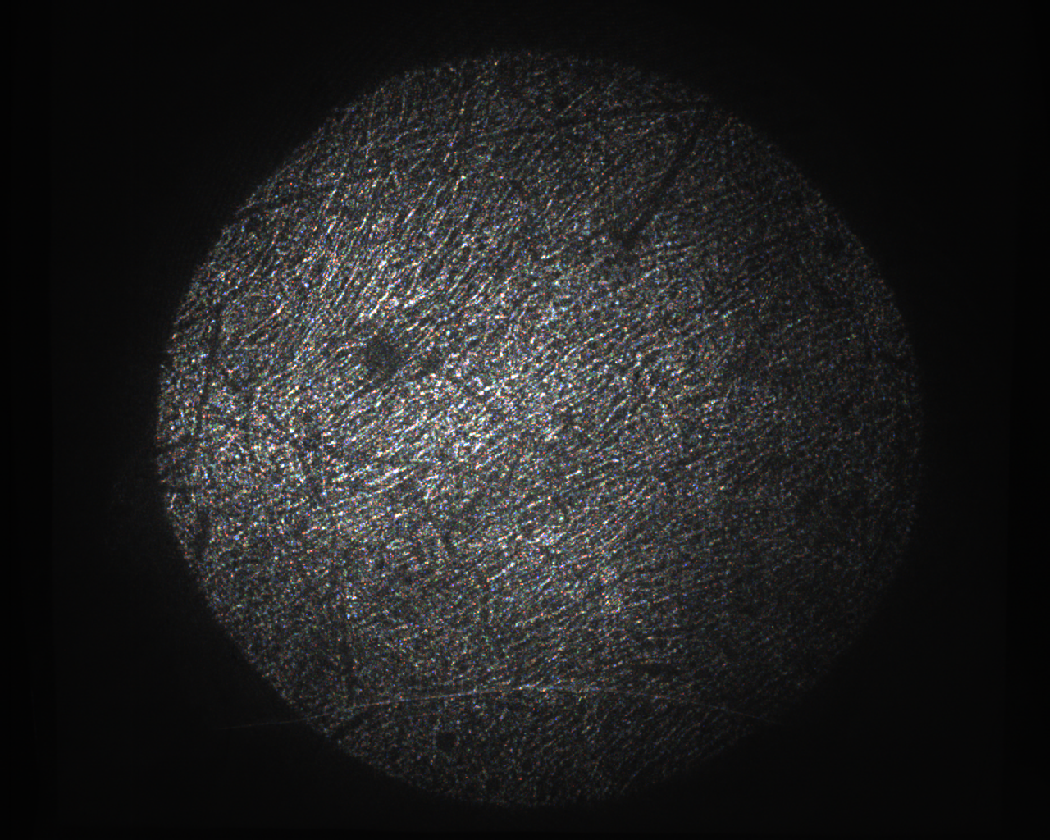
\includegraphics[width=.5\textwidth]{5.20/9.pdf}
\end{center}
    此图为厚度$d=\SI{4}{mm}$,加热电流$I=\SI{0.201}{A}$, 下界面温度为25.7摄氏度,
    上界面温度为21.4摄氏
    度时的斑图图样,可以看到,此时非线性对流现象尚未出现.

\begin{center}
    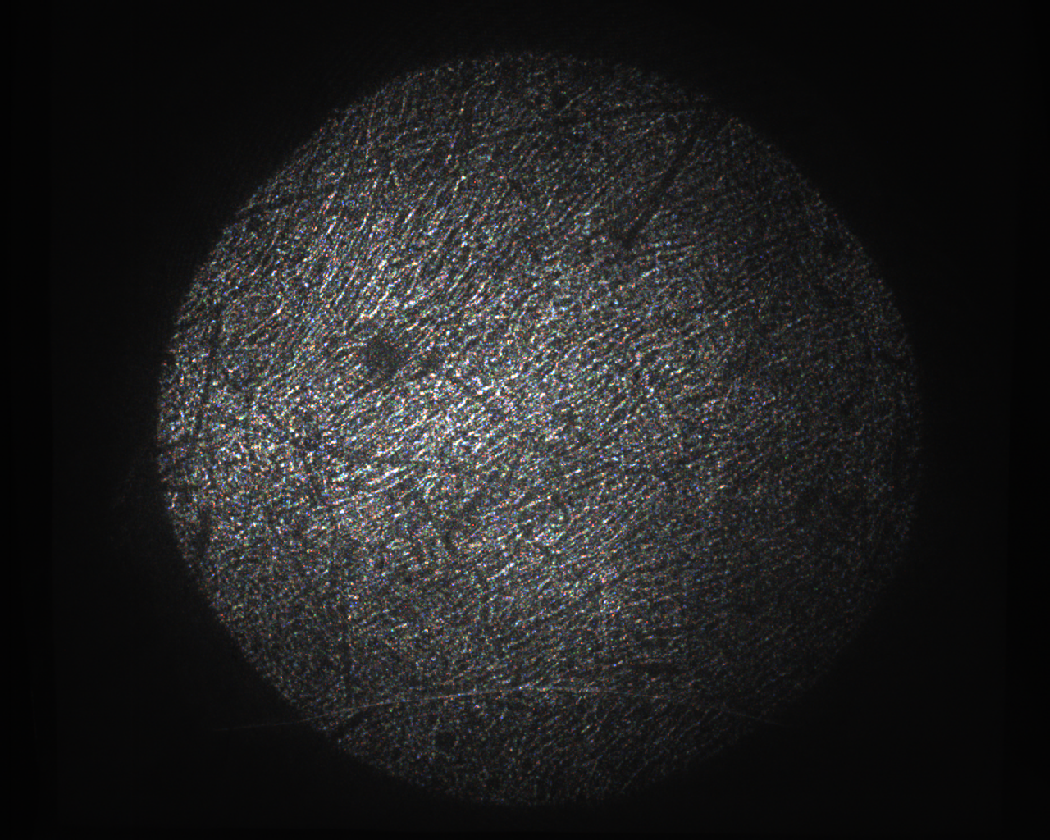
\includegraphics[width=.5\textwidth]{5.20/10.pdf}
\end{center}
    此图为厚度$d=\SI{4}{mm}$,加热电流$I=\SI{0.30}{A}$, 下界面温度为24.5摄氏度,
    上界面温度为21.0摄氏
    度时的斑图图样,可以看到,此时非线性对流现象尚未出现.

\begin{center}
    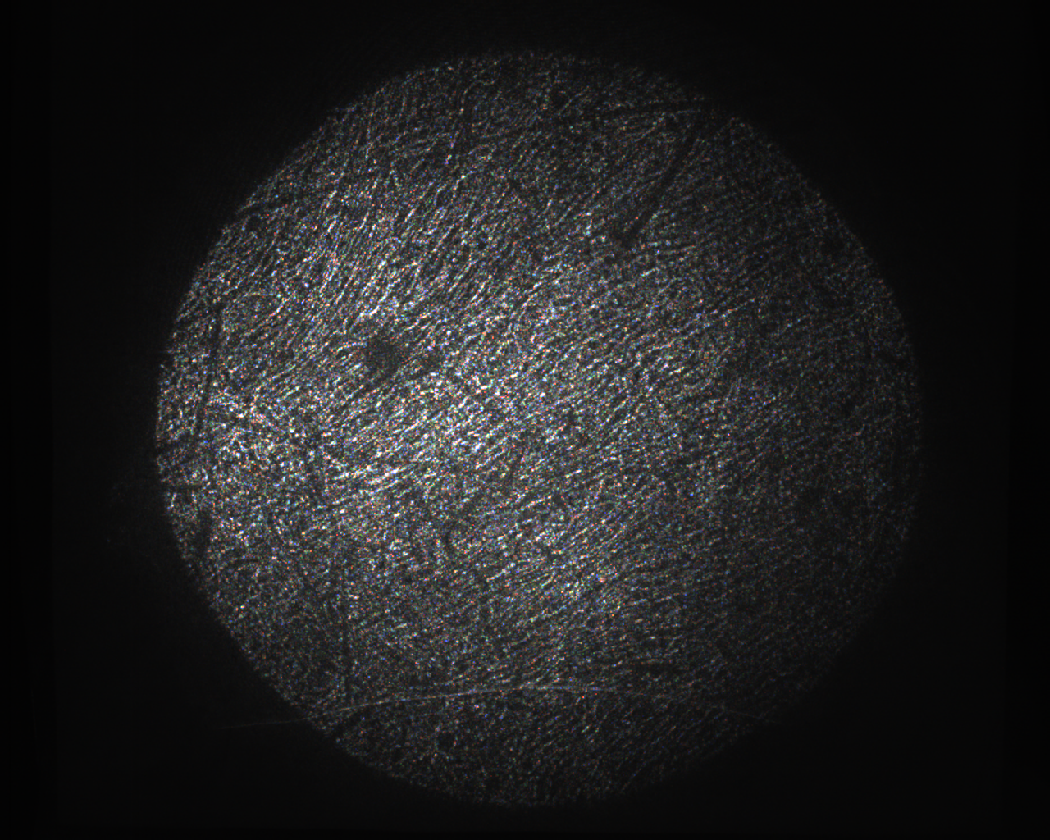
\includegraphics[width=.5\textwidth]{5.20/11.pdf}
\end{center}
    此图为厚度$d=\SI{4}{mm}$,加热电流$I=\SI{0.401}{A}$, 下界面温度为25.5摄氏度,
    上界面温度为20.7摄氏
    度时的斑图图样,可以看到,此时黑白相间的非线性对流斑图已经隐约可见.

\begin{center}
    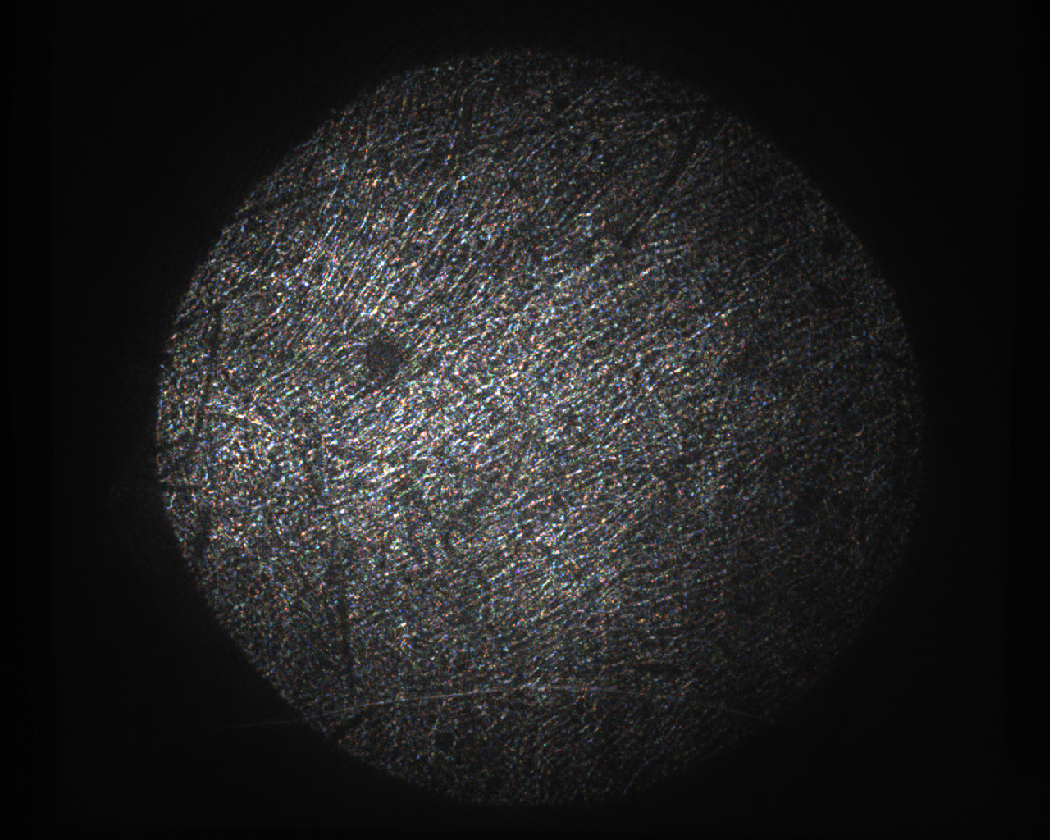
\includegraphics[width=.5\textwidth]{5.20/12.pdf}
\end{center}
    此图为厚度$d=\SI{4}{mm}$,加热电流$I=\SI{0.500}{A}$, 下界面温度为27.2摄氏度,
    上界面温度为21.2摄氏
    度时的斑图图样,可以看到,此时斑图变得更加明显

\begin{center}
    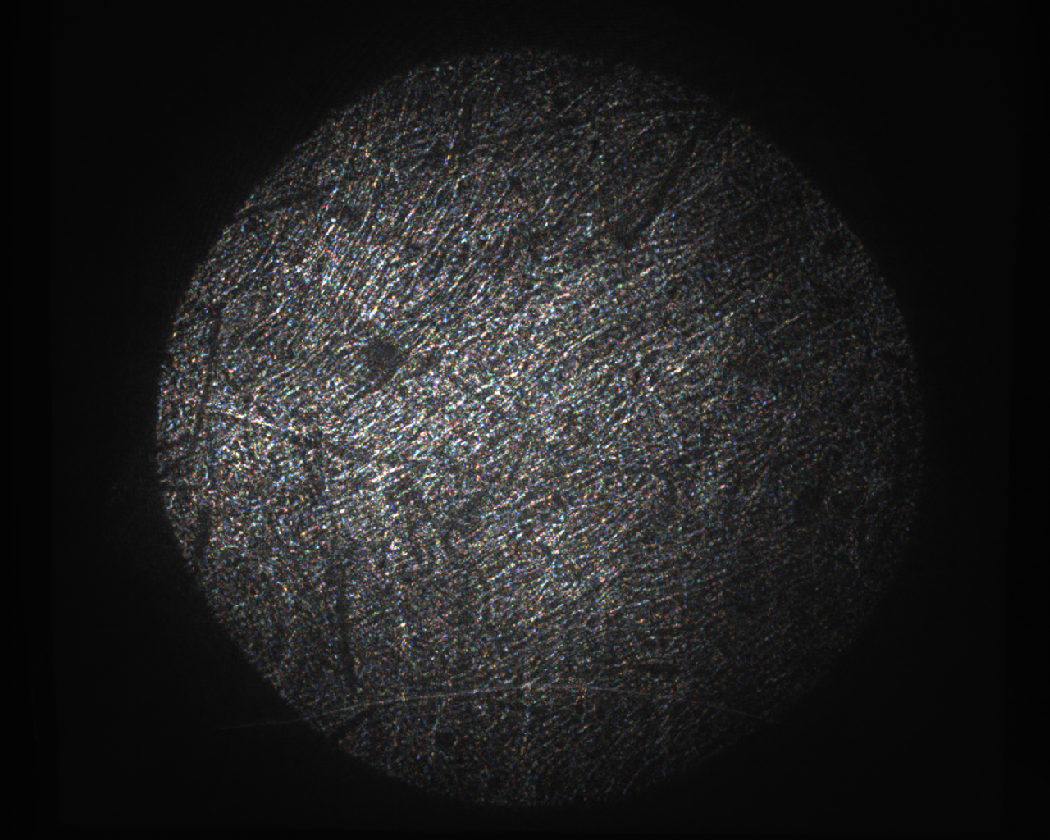
\includegraphics[width=.5\textwidth]{5.20/13.pdf}
\end{center}
    此图为厚度$d=\SI{4}{mm}$,加热电流$I=\SI{0.600}{A}$, 下界面温度为29.3摄氏度,
    上界面温度为22.9摄氏
    度时的斑图图样,可以看到,此时斑图变得更加明显.

\begin{center}
    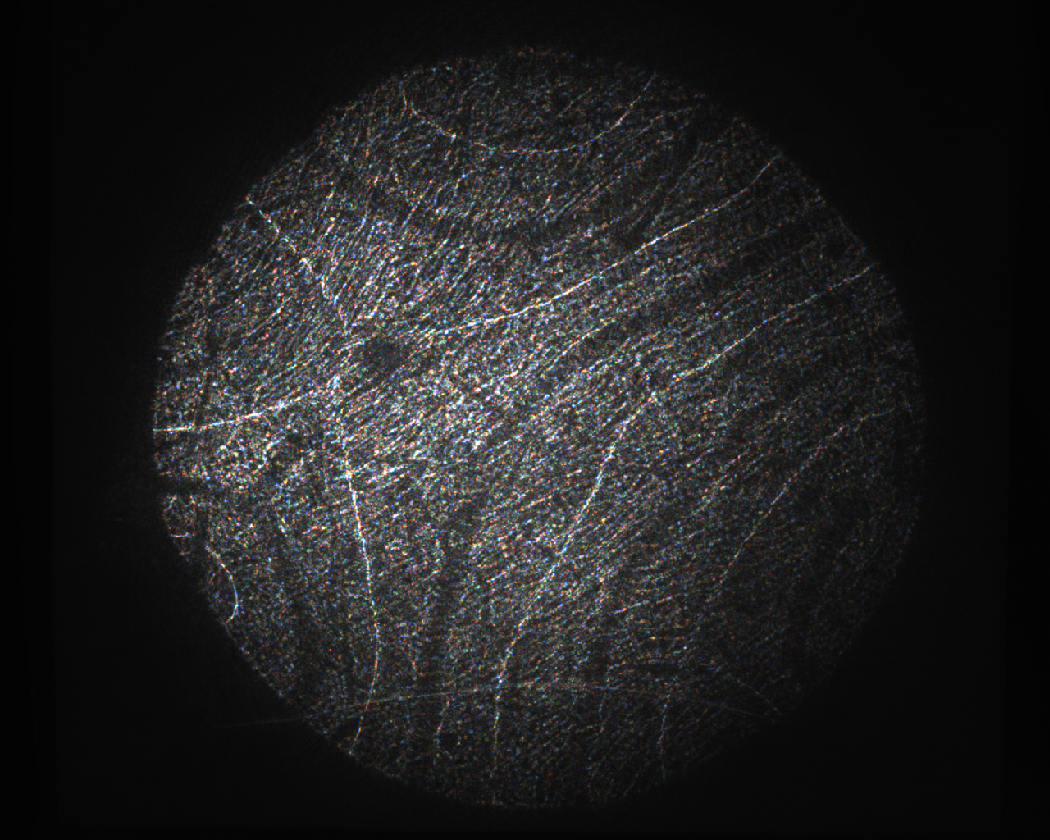
\includegraphics[width=.5\textwidth]{5.20/14.pdf}
\end{center}
    此图为厚度$d=\SI{4}{mm}$,加热电流$I=\SI{0.800}{A}$, 下界面温度为33.3摄氏度,
    上界面温度为23.6摄氏
    度时的斑图图样,可以看到,此时斑图变得更加明显.

\begin{center}
    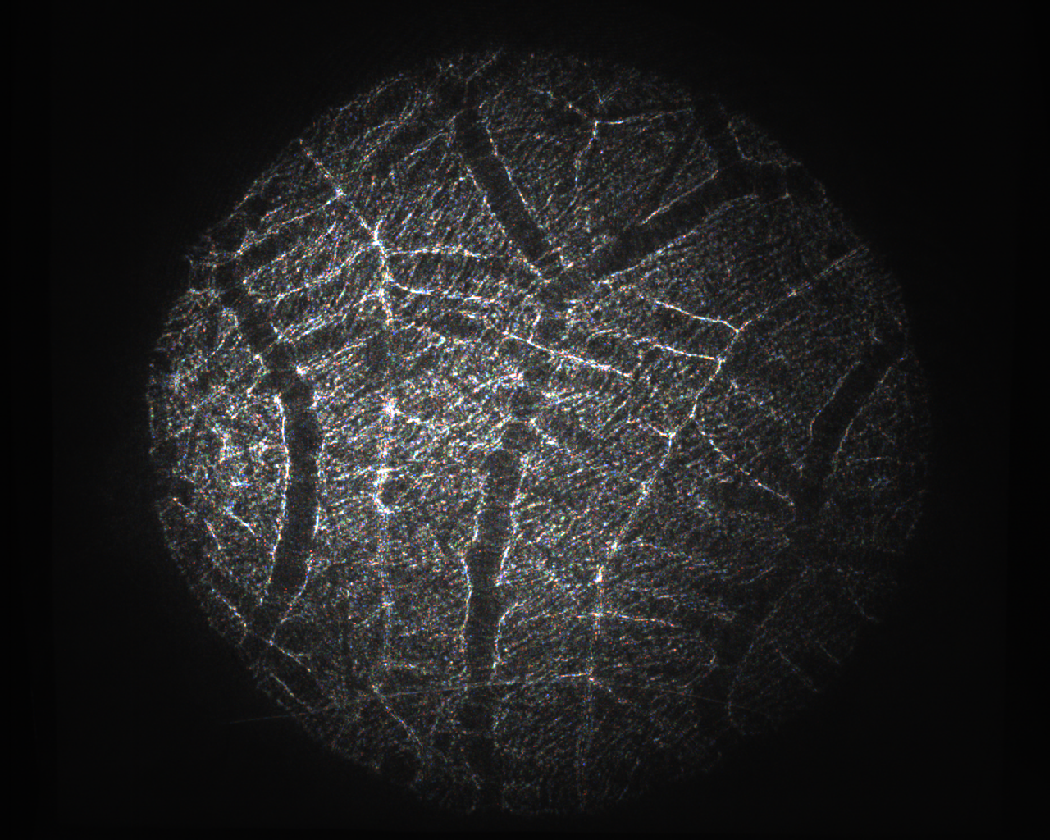
\includegraphics[width=.5\textwidth]{5.20/15.pdf}
\end{center}
    此图为厚度$d=\SI{4}{mm}$,加热电流$I=\SI{1.000}{A}$, 下界面温度为41.5摄氏度,
    上界面温度为26.8摄氏
    度时的斑图图样,可以看到,此时系统的对流已经失稳,对流斑图开始剧烈地随时间演化.

\begin{center}
    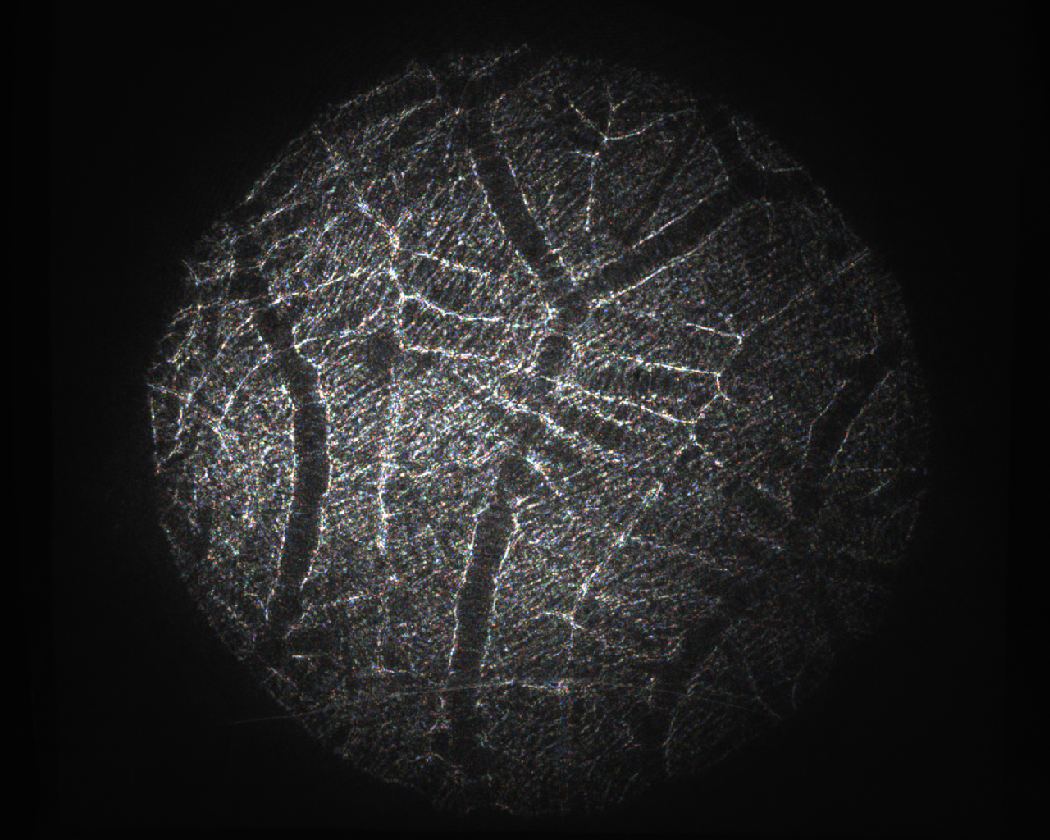
\includegraphics[width=.5\textwidth]{5.20/16.pdf}
\end{center}
    此图为厚度$d=\SI{4}{mm}$,加热电流$I=\SI{1.000}{A}$, 下界面温度为41.5摄氏度,
    上界面温度为26.8摄氏
    度时的斑图图样,可以看到,此时系统的对流已经失稳,对流斑图开始剧烈地随时间演化.

\begin{center}
    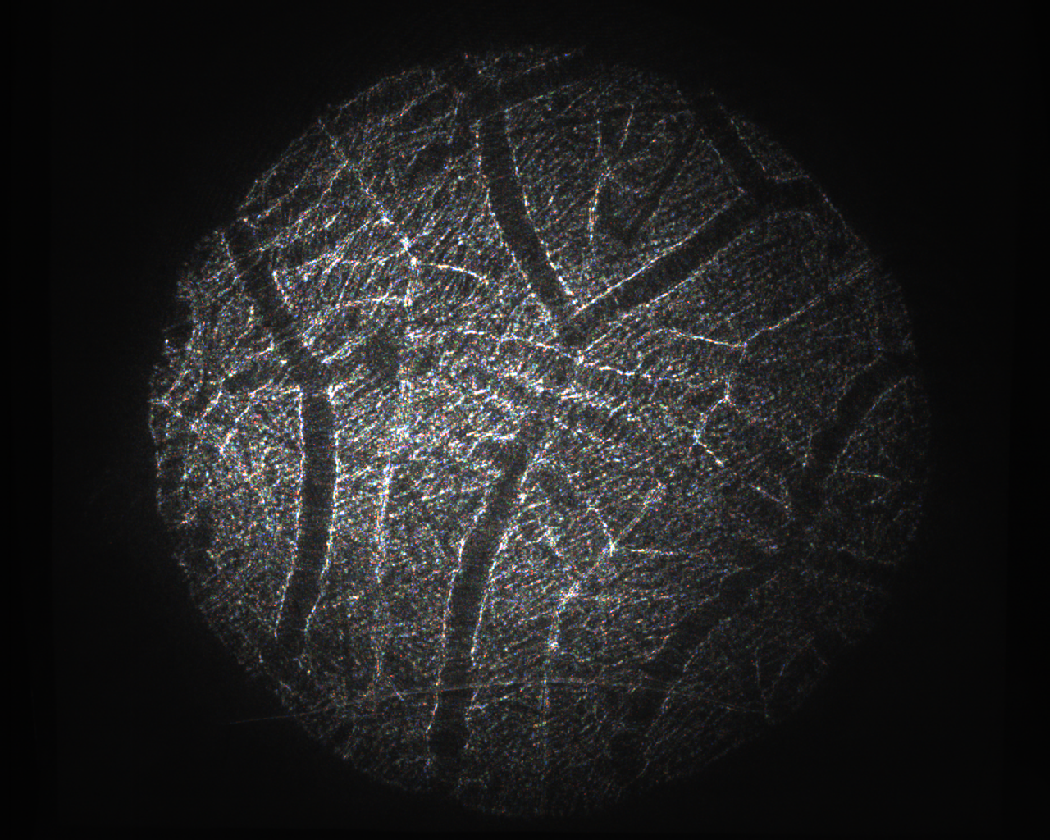
\includegraphics[width=.5\textwidth]{5.20/17.pdf}
\end{center}
    此图为厚度$d=\SI{4}{mm}$,加热电流$I=\SI{1.000}{A}$, 下界面温度为41.8摄氏度,
    上界面温度为27.4摄氏
    度时的斑图图样,可以看到,此时系统的对流已经失稳,对流斑图开始剧烈地随时间演化.

\begin{center}
    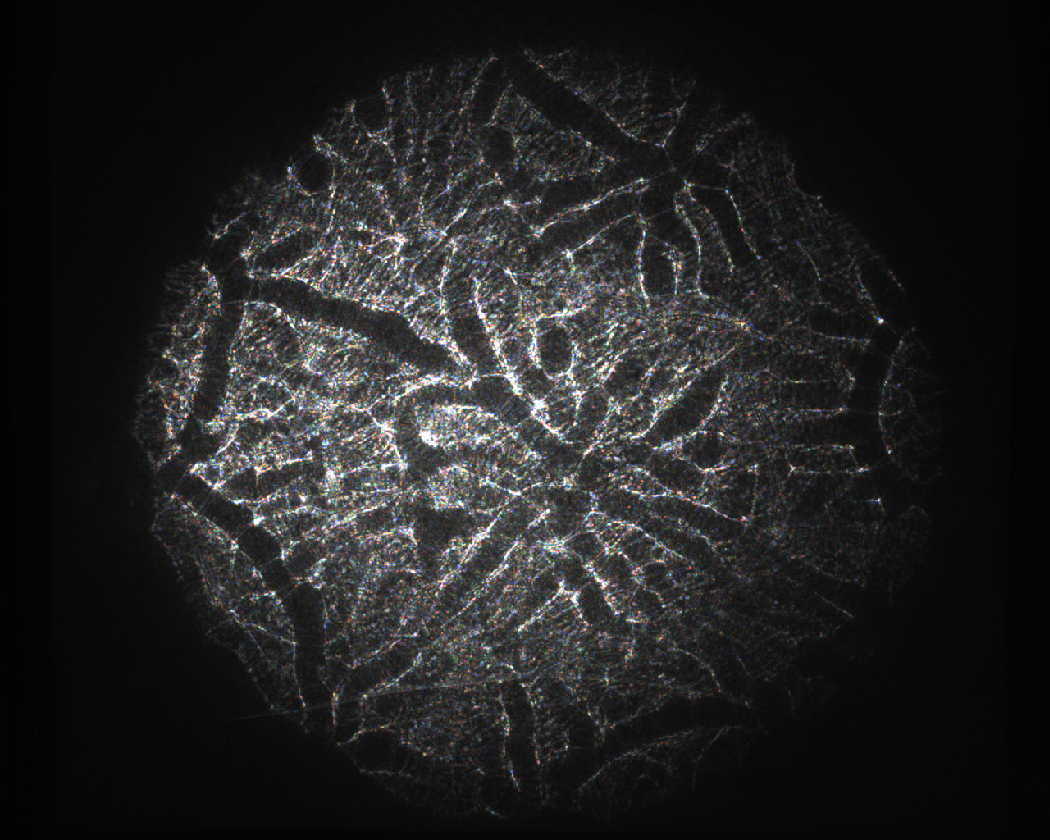
\includegraphics[width=.5\textwidth]{5.20/18.pdf}
\end{center}
    此图为厚度$d=\SI{4}{mm}$,加热电流$I=\SI{1.200}{A}$, 下界面温度为50.4摄氏度,
    上界面温度为31.8摄氏
    度时的斑图图样,可以看到,此时系统的对流已经失稳,对流斑图开始剧烈地随时间演化.

\begin{center}
    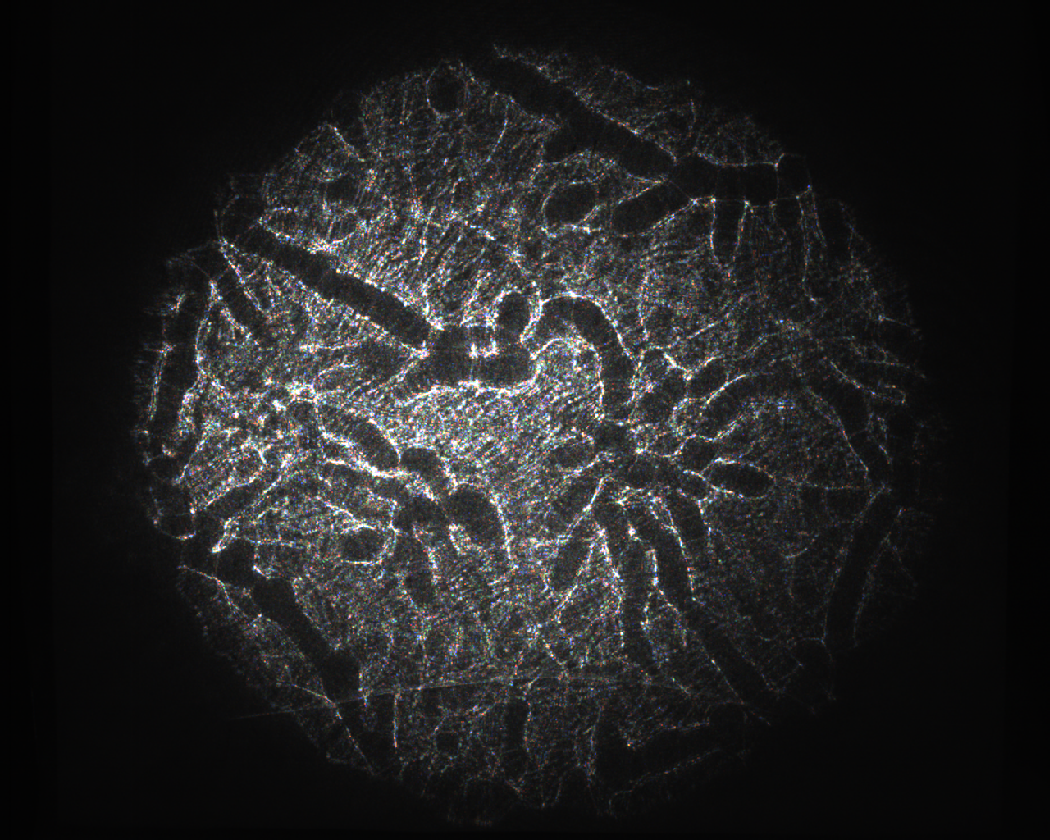
\includegraphics[width=.5\textwidth]{5.20/19.pdf}
\end{center}
    此图为厚度$d=\SI{4}{mm}$,加热电流$I=\SI{1.200}{A}$, 下界面温度为50.5摄氏度,
    上界面温度为31.5摄氏
    度时的斑图图样,可以看到,此时系统的对流已经失稳,对流斑图开始剧烈地随时间演化.

\begin{center}
    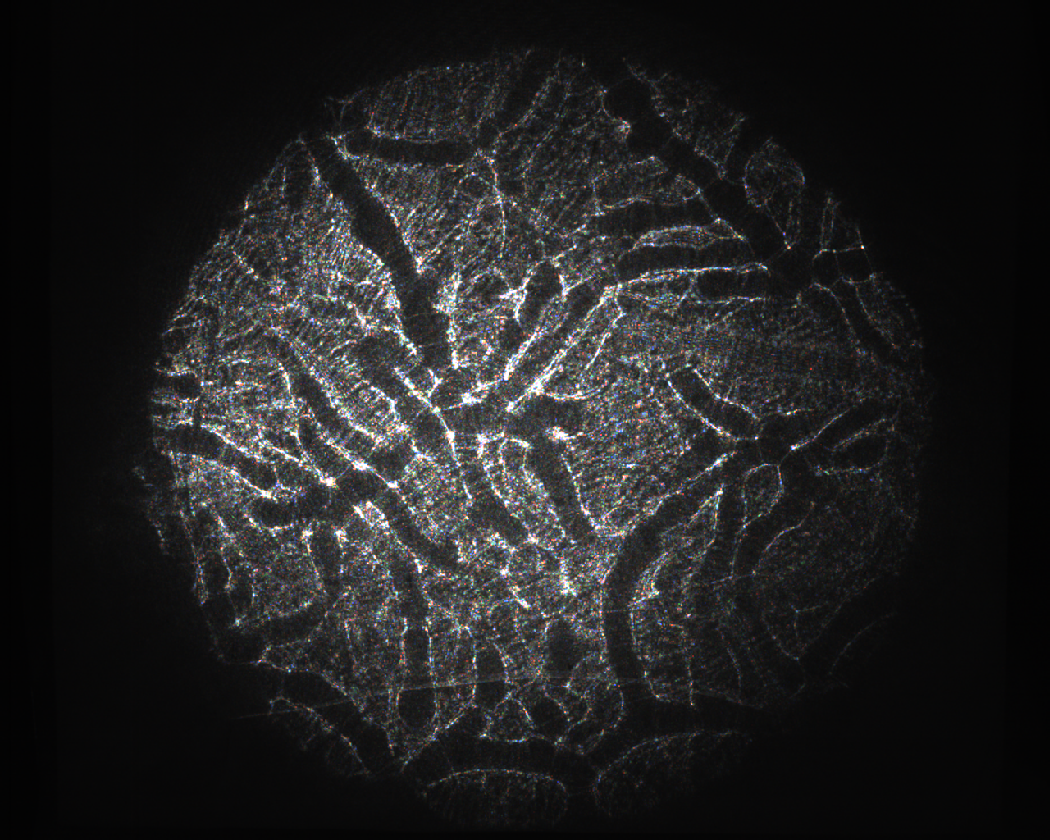
\includegraphics[width=.5\textwidth]{5.20/20.pdf}
\end{center}
    此图为厚度$d=\SI{4}{mm}$,加热电流$I=\SI{1.200}{A}$, 下界面温度为50.5摄氏度,
    上界面温度为31.1摄氏
    度时的斑图图样,可以看到,此时系统的对流已经失稳,对流斑图开始剧烈地随时间演化.

\section{结论}

实验验证了非线性斑图理论的相关预言,并且粗略地验证了瑞利数与温度差之间的关系.

\section{致谢}


感谢周路群老师在实验中严谨而细致的指导.

\begin{thebibliography}{}
\bibitem{Script} 非平衡实验讲义, 近代物理实验讲义,  北京大学物理学院.
\bibitem{NCP} 新概念物理学教程, 热学, 赵凯华, 北京大学出版社.
\bibitem{ZKH} 定性与半定量物理学, 赵凯华, 北京大学出版社.
\end{thebibliography}

\clearpage
\appendix
\section{思考题}

\begin{enumerate}
    \item 应当是黑色部分对应温度较低部分,白色部分对应温度较高部分.
    \item 斑图出现的临界点即是随着温差值的变化,斑图图样中出现黑白相间条纹的温度
        差值.
    \item 临界点应当变小,而且应当大约是之前值的八分之一
    \item 可以通过与光束的半径作相对比较而确定空间尺度.
    \item 水层厚度越大,特征尺度也越大.
\end{enumerate}


\end{document}
